\begin{figure}[!htbp]
  \centering
  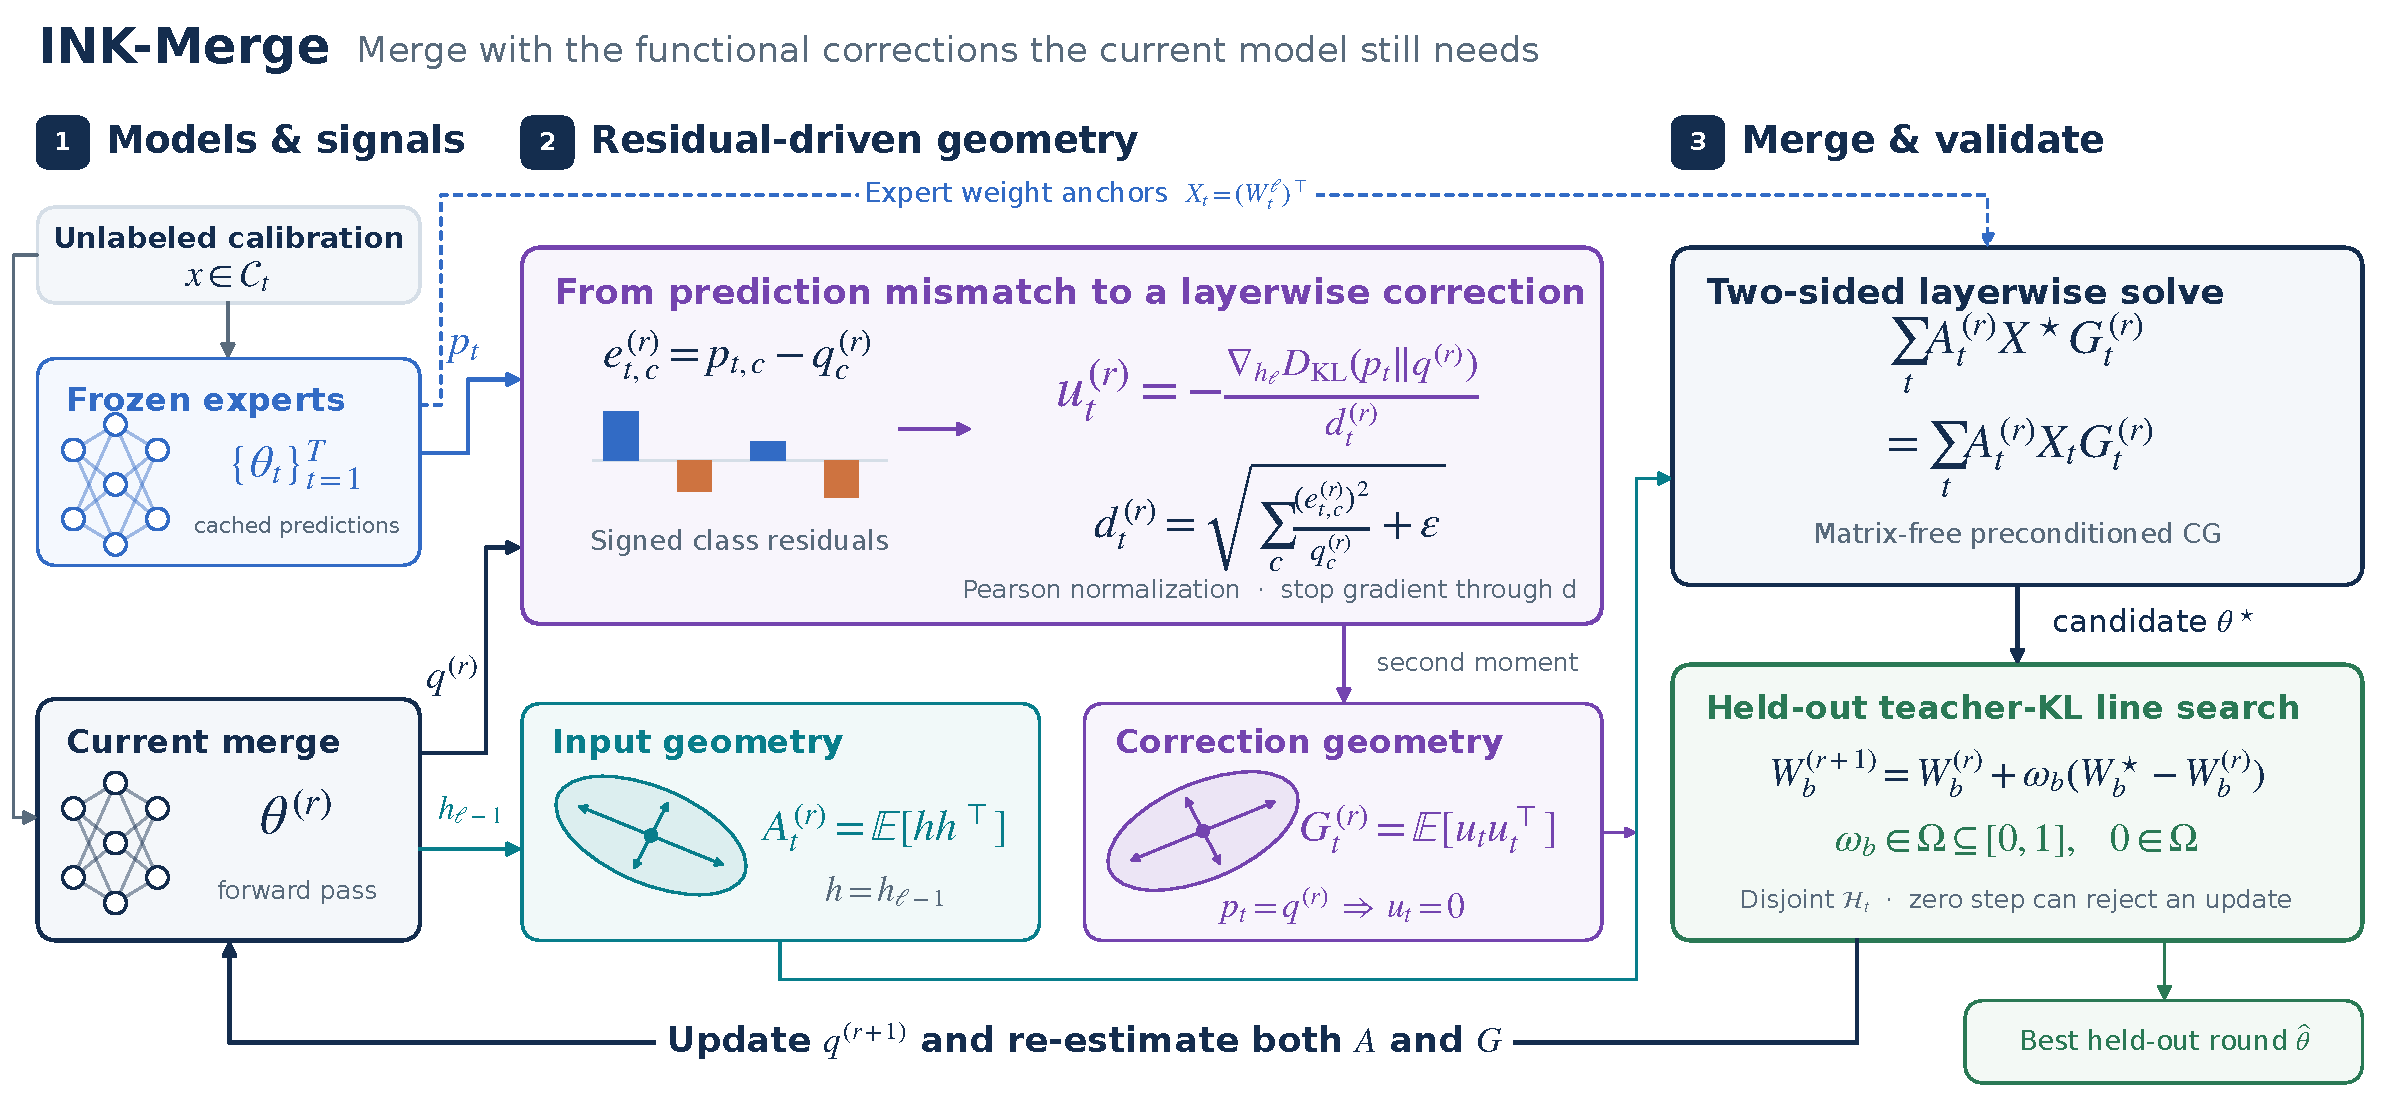
\includegraphics[width=\linewidth]{figures/ink_method_overview.pdf}
  \caption{\method{} 方法总览，对应式~(\ref{eq:ink-dynamic-geometry})。\textbf{1}~冻结专家提供软预测 $p_t$ 与权重锚点 $X_t$，当前模型 $\theta^{(r)}$ 给出 $q^{(r)}$ 与激活 $h_{\ell-1}$。\textbf{2}~类别残差经教师--学生 KL 负梯度与 Pearson 归一化得到层级修正 $u_t^{(r)}$；其二阶矩 $G_t^{(r)}$ 与输入二阶矩 $A_t^{(r)}$ 构成随 $\theta^{(r)}$ 变化的双侧几何。\textbf{3}~矩阵自由预条件共轭梯度求解候选权重，留出教师 KL 选择块级步长（含零步长拒绝），随后重估 $A$ 与 $G$ 并迭代，最终取留出 KL 最小的轮次。图中省略层下标 $\ell$，$G_t^{(r)}$ 简记 $G_{t,\mathrm{ink}}^{\ell,(r)}$，椭圆仅示意几何方向。}
  \label{fig:ink-overview}
\end{figure}
